
\begin{comment}

\begin{tikzpicture}
%\onslide<2-> \node[align=center] at (3.5,4.5) { \textcolor{navyblue}{Billing Records} };
\onslide<2->\node[overlay] at (5, 3.5) {    \begin{minipage}{1\textwidth} { \small
        \textcolor{navyblue}{Transaction Records}
        \vspace{.1cm}
        \begin{itemize}
          \itemsep0em 
    \item 1.5 mil. connections (GPS locations)    
    \item Monthly 2008-2015
        \end{itemize} }
    \end{minipage}};


\onslide<3->\node[overlay] at (5, -1.5) {    \begin{minipage}{1\textwidth} { \small
        {Connection Survey}
     %   \vspace{.05cm}
        \begin{itemize}
          \itemsep0em 
    \item 48,000 connections
    \item HHs and people served \\ (demographics for owner)
  \end{itemize}
        }
    \end{minipage}};

\onslide<4->\node[overlay] at (12, -1.5) {    \begin{minipage}{1\textwidth} { \small
        \textcolor{navyblue}{Census 2010}
     %   \vspace{.05cm}
        \begin{itemize}
          \itemsep0em 
    \item Unconnected HHs \\
      (demographics)
    \item Merge geographically
  \end{itemize}
        }
    \end{minipage}};

%\onslide<2-> \node[align=center] at (7.5,4.5) { \textcolor{navyblue}{Census 2010} };


\onslide<1->\node[align=center] at (3.5,2.2) {{\small Connections}};
\onslide<1->\node[align=center] at (7.5,2.8) {{\small Vendor}};
\onslide<1->\node[align=center] at (4.5,-.5) {{\small Households}};


\onslide<+->\draw [color=black, fill=none, radius=.2,line width=0.5mm]  (2, 2) circle[];  
\draw [color=black, fill=black, radius=.2]  (1, .5) circle[]; 
\draw [line width=0.5mm,
  ->,  shorten <=.45cm + \pgflinewidth,  shorten >=.45cm + \pgflinewidth,
] (1, .5) -- (2, 2);
\draw [color=black, fill=none, radius=.2,line width=0.5mm]  (5, 2) circle[];  
\draw [color=black, fill=black, radius=.2] (4, 0) circle[];  
\draw [line width=0.5mm,
  ->,  shorten <=.45cm + \pgflinewidth,  shorten >=.45cm + \pgflinewidth,
] (4, 0) -- (5, 2);
\draw [color=black, fill=black, radius=.2] (5.5, .5) circle[]; 
\draw [line width=0.5mm,
  ->,  shorten <=.45cm + \pgflinewidth,  shorten >=.45cm + \pgflinewidth,
] (5.5, .5) -- (5, 2);
\draw [color=black, fill=none,line width=0.5mm]  (7.75, 2.25)--(7.25, 2.25)--(7.25, 1.75)--(7.75, 1.75)--cycle ;  
\draw [color=black, fill=black, radius=.2]  (7.5, 0) circle[]; 
\draw [line width=0.5mm,
  ->,  shorten <=.45cm + \pgflinewidth,  shorten >=.45cm + \pgflinewidth,
] (7.5, 0) -- (7.5, 2);
\end{tikzpicture}
\end{center}
\end{frame}




\begin{enumerate}
  \item \textbf{Seller Identity:} match government names and housing authorities in seller-names from transactions 
  \begin{tabu}{lc}
\toprule
 Seller Name & Observations \\
\midrule
City Of Johannesburg Metropolitan Municipality & 29,087  \\
City Of Johannesburg & 27,672  \\
City Of Tshwane Metropolitan Municipality & 24,780  \\
Ekurhuleni Metropolitan Municipality & 21,758  \\
Gauteng Provincial Housing Advisory Board & 13,058  \\
{\bf Total Observations }& {\bf 549,704}  \\
\bottomrule
\end{tabu}

  \item \textbf{Subsidy Value:} exclude purchase prices R50,000 above subsidy value
  \item \textbf{Pre-Existing Formal Dwellings:} exclude land plots with formal structures in 2001 building census
  \item \textbf{Spatial Clustering:} collect nearby houses into projects with density-based clustering algorithm
  \item \textbf{Temporal Clustering:} include cluster with $>$50\% of transactions during modal year
\end{enumerate}

\begin{itemize}
  \item do formal comparison to GCRO or 
\end{itemize}

% $\node[overlay,anchor=west,align=left] at (0, -2) {   \onslide<3>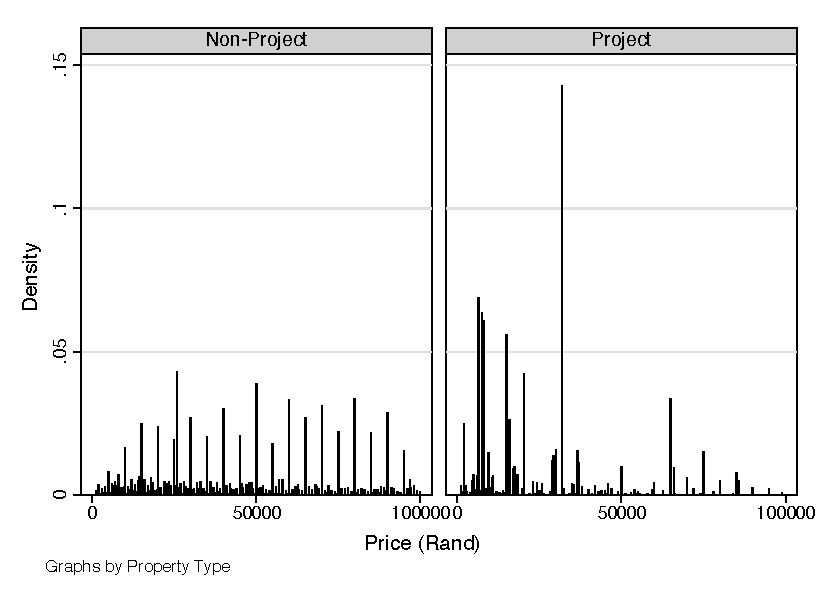
\includegraphics[scale=.5]{price_histogram.pdf} };


\end{comment}